\documentclass{article}
\usepackage[ngerman]{babel}
\usepackage{amsmath}
\usepackage{graphicx}
\usepackage{float}
\usepackage{xcolor}
\usepackage{mhchem}
\title{Physik Skript}
\author{Linus Hesmert}
\date{\today}

\begin{document}

\maketitle
\tableofcontents
\newpage

\section{Mechanik}
\subsection{Kinematik}
Es geht um die Beschreibung der Bewegung, nicht um die Ursachen der Bewegung

\subsubsection{Ort, Geschwindigkeit und Beschleunigung}
Für $v=const$ gilt:
\begin{align}
    v=\frac{\Delta x}{\Delta t}
\end{align}
für $v\neq const$ gilt, dass die Geschwindigkeit $v$ in abhängigkeit
zur Zeit steht, also $v: t\to v$. Dafür geht $\Delta t$ gegen Null.
\begin{equation}
    v(t)=\lim_{\Delta t\to 0} \frac{\Delta x}{\Delta t}=\frac{dx}{dt}=\dot{x}(t)
\end{equation}
Somit entspricht die Geschwindigkeit der zeitlichen Ableitung der Ortsfunktino.
Dies ist Äquivalent zur Tangentensteigung der Ortsfunktion $x(t)$.\\

\noindent Bei der Beschleunigung $a(t)$ geht es darum, wie schnell sich die Geschwindigkeit
in Abhängigkeit zur Zeit ändert. Dies ist Äquivalent zur zeitlichen Ableitung der Geschwindigkeit
und zur zweiten zeitlichen Ableitung der Ortsfunktion.
\[a(t)=\dot{v}(t)=\ddot{x}(t)\]

\subsubsection{Herleitung des Weg Zeit Gesetz}
Beim Weg Zeit Gesetz gilt: $a=const$
\begin{align}
    a(t)&:=\dot{v}(t)\\
    \int a(t)dt&=\int \dot{v}(t)dt \quad \text{da }a=const\\
    a\cdot \int dt&=\int \dot{v}(t)dt\\
    a\cdot t+v_0&=v(t)\\
    \int a\cdot t \ dt+ \int v_0 \ dt&=\int \dot{x}(t) dt\\
    \frac{1}{2}at^2+v_0t+x_0&=x(t)
\end{align}
$v_0$ (Anfangsgeschwindigkeit) und $x_0$ (Anfangsweg) sind Integrationskonstanten.

\subsubsection{Bestimmung der Ortskurve aus der Beschleunigung}
Aus der Ableitung der Geschwindigkeit folgt:
\begin{align}
    dv(t)=a(t)dt
\end{align}
Durch Integration im Intervall $[t_0,t]$ folgt
\begin{equation}
    \Delta v=\int_{t_0}^{t} a(t')dt'
\end{equation}
das $t'$ und $dt'$ ist lediglich Formal, da es sonst eine Verwechslung mit den Integrationsgrenzen geben könnte.\\
Durch Addition der Anfangsgeschwindigkeit $v_0$ folgt aus $\Delta v$ dann $v(t)$:
\begin{equation}
    v(t)=\int_{t_0}^{t}a(t')dt' + v_0
\end{equation}
Gleiches gilt auch für den Ort:
\begin{equation}
    x(t)=\int_{t_0}^{t} v(t')dt' + x_0
\end{equation}

\subsubsection{Der Freie Fall}
Ein Körper startet aus der Ruhe ($v_0=0$) von der Höhe $h_0$ und prallt nach einer gewissen Zeit $t$ auf den Boden auf ($h=0$)
\begin{align}
    v(t)=\int_{t_0}^{t}a\ dt'+v_0
\end{align}
Da wir die Zeit selbst festlegen können ist $t_0=0$. Die Beschleunigung des Körpers entspricht der negativen Erdbeschleunigung $a=-g$.
Die Erdbeschleunigung ist negativ, da der Körper in die negative Richtung der Achse fällt. Da der Körper aus der Ruhe startet gilt $v_0=0$
\begin{align}
    v(t)&=\int_{0}^{t}(-g)\ dt'\\
    &=-gt \label{Freier_Fall_v}
\end{align}
Um nun auf den Weg, also die Höhe des Körpers zu kommen, muss nochmal Integriert werden.
\begin{align}
    h(t)&=\int_{t_0}^{t}-gt'\ dt'+h_0\\
    &=\int_{0}^{t}-gt'\ dt' + h_0\\
    &=-\frac{gt^2}{2}+h_0\\
    &=h_0-\frac{gt^2}{2}
\end{align}
Um nun zum Beispiel auf die Zeit des Aufpralls (h=0) zu kommen folgt
\begin{align}
    0=h_0-\frac{gt^2}{2}\\
    t=\sqrt{\frac{2h_0}{g}}
\end{align}
Um nun zum Beispiel auf die Geschwindigkeit zum Zeitpunkt des Aufpralls zu kommen kann die Zeit zum Aufprall in Gleichung \ref{Freier_Fall_v} eingesetzt werden.\\
Die Funktion von $h(t)$ ist in Abbildung \ref{fig:Freier Fall h(t)} zu sehen.
\begin{figure}[H]  % Bildumgebung
    \centering      % Bild zentrieren
    \includegraphics[width=0.7\textwidth]{Freier Fall Geschwindigkeit Plot.png} % Bild einfügen
    \caption{Plot der Funktion $h(t)$ mit $h_0=10$} % Bildunterschrift
    \label{fig:Freier Fall h(t)} % Label für Verweise
\end{figure}

\subsubsection*{Im Dreidimensionalen Raum}
Gleiches gilt auch im Dreidimensionalen Raum. Die Bewegung wird nun als Vektor dargestellt. Alle drei richtungen des Vektors
sind unabhängig voneinander. Betrachtet wird die einzelne Bewegung über die Kombination der Einheitsvektoren ($\hat{\imath},\hat{\jmath},\hat{k}$)
\begin{align}
    \vec{r}(t)=
    \left(\begin{matrix}
        x(t)\\
        y(t)\\
        z(t)
    \end{matrix}\right)
    =x(t)\cdot \hat{\imath}+y(t)\cdot \hat{\jmath}+z(t)\cdot \hat{k}
\end{align}
Für die Geschwindigkeit gilt dann:
\begin{align}
    \vec{v}(t)&=\frac{d\vec{r}(t)}{dt}=\frac{d\vec{x}(t)}{dt}\cdot \hat{\imath}+\frac{d\vec{y}(t)}{dt}\cdot \hat{\jmath}+\frac{d\vec{z}(t)}{dt}\cdot \hat{k}\\
    &=v_x(t)\cdot \hat{\imath}+v_y(t)\cdot\hat{\jmath}+v_z(t)\cdot\hat{k}\\
    &=\left(\begin{matrix}
        v_x(t)\\v_y(t)\\v_z(t)
    \end{matrix}\right)
\end{align}
Gleiches gilt auch für die Beschleunigung. Beim Integrieren läuft alles äquivalent zum differenzieren.

\subsubsection{Schiefer Wurf}
Ein Körper wird mit einer Startgeschwindigkeit ($v_0$) unter einem Winkel $\alpha$ (zur Horizontalen) abgeworfen.\\
Man setzt die Abwurfpositionen gleich dem Ursprung $\Rightarrow x_0=0$ und $y_0=0$
\begin{figure}[H]  % Bildumgebung
    \centering      % Bild zentrieren
    \includegraphics[width=0.6\textwidth]{Schräger Wurf v_0.png} % Bild einfügen
    \caption{Schräger Wurf mit $v_0$ und $\alpha$} % Bildunterschrift
    \label{fig:Schräger Wurf} % Label für Verweise
\end{figure}
\noindent Die Komponenten des Vektors $v_0$ können durch polarkoordinaten zerlegt werden.
\begin{align}
    \vec{v_0}=\left(\begin{matrix}
        v_{x,0}\\v_{y,0}
    \end{matrix}\right)
    =\left(\begin{matrix}
        |v_0|\cdot \cos(\alpha)\\
        |v_0|\cdot \sin(\alpha)
    \end{matrix}\right)\label{Schräger Wurf polar}
\end{align}
Auf den Körper wirkt die negative Erdbeschleunigung in $y$-Richtung.
\begin{align}
    \vec{a}=\left(\begin{matrix}
        0\\-g
    \end{matrix}\right)
\end{align}\\
Nun kann man wie gewohnt die Beschleunigung in $y$-Richtung integrieren um die Geschwindigkeit der $y$-Richtung zur erhalten. Da wir in $t_0=0$ starten können wir dies direkt als Integrationsgrenze schreiben.
\begin{align}
    v_y(t)&=\int_{0}^{t}(-g)\ dt' + v_{y,0}\\
    &=v_{y,0}-gt
\end{align}
$v_{y,0}$ erhalten wir aus der Anfangsgeschwindigkeit durch die Komponentenzerlegung in \ref{Schräger Wurf polar}.\\
Die Geschwindigkeit kann nun weiter Integriert werden um die Ortskurve für $y$ zu erhalten.
\begin{align}
    y(t)&=\int_{0}^{t}v_y(t')\ dt'\\
    &=\int_{0}^{t}(v_{y,0}-gt')\ dt'\\
    &=v_{y,0}\cdot t-\frac{1}{2}gt^2
\end{align}
Nun können, wie beim Freien Fall, sonstige Werte berechnet werden. So zum Beispiel die Zeit $T$ beim Aufprall auf den Boden.\\
Dafür gilt $y(T)=0$
\begin{align}
    0&=v_{y,0}T-\frac{1}{2}gT^2\\
    0&=t(v_{y,0}-\frac{1}{2}gT)\\
    \Longleftrightarrow 0&=v_{y,0}-\frac{1}{2}gT \label{v_y,0}\\
    \Longleftrightarrow T&=\frac{2\cdot v_{y,0}}{g}
\end{align}
Die maximale Höhe kann berechnet werden mit der Bedingung, dass die Geschwindigkeit in diesem Punkt gleich Null sein muss.\\
Also folgt $v_y=0$
\begin{align}
    0&=v_{y,0}-gt\\
    \Longleftrightarrow t&=\frac{v_{y,0}}{g}\label{maxHöhe}
\end{align}
Durch einsetzen der Gleichung \ref{v_y,0} in Gleichung \ref{maxHöhe} folgt:
\begin{align}
    t=\frac{T}{2}
\end{align}
$T$ ist die Zeit bei der der Körper den Boden berührt. Hiermit ist gezeigt worden, dass die maximale Höhe bei der hälfte der Zeit der reicht ist.\\

Die Geschwindigkeit in $x$-Richtung bleibt unverändert. Somit gilt:
\begin{align}
    v_x=v_{x,0}
\end{align}
Das kann wiederum Integriert werden um $x(t)$ zu erhalten.
\begin{align}
    x(t)=\int_{0}^{t}v_{x,0}\ dt' + x_0
\end{align}
Da $x_0=0$ folgt:
\begin{align}
    x(t)=v_{x,0}\cdot t \label{Schiefer Wurf x(t)}
\end{align}
Mit dieser Gleichung können wir die Wurfweite Berechnen, in dem wir $t=T$ einsetzen, also die Zeit bei der der Körper am Boden
aufkommt. \\
Mit $T=\frac{2\cdot v_{y,0}}{g}$ in Gleichung \ref{Schiefer Wurf x(t)} folgt:
\begin{align}
    l:=x(T)=\frac{2\cdot v_{x,0}\cdot v_{y,0}}{g}
\end{align}
$l$ ist nun definiert als die Funktion der Wurfweite.\\
Nun könnte man die größte Wurfweite für einen Abwurfwinkel $\alpha$ berechnen. Hierfür kann man die erste Ableitung nach $\alpha$ der Wurfweite $l=x(T)$ gleich Null setzen (Extrema).
\begin{align}
    &\frac{dl}{d\alpha}=0\\
    0=\frac{d}{d\alpha}&\left(\frac{2\cdot v_{x,0}\cdot v_{y,0}}{g}\right)
\end{align}
Durch $v_{x,0}=v_0\cdot \cos(\alpha)$ und $v_{y,0}=v_0\cdot \sin(\alpha)$ folgt:
\begin{align}
    0&=\frac{d}{d\alpha}\left(\frac{2\cdot v^2_0\cdot \cos(\alpha)\cdot \sin(\alpha)}{g}\right)\\
    0&=\frac{2v_0^2}{g}\cdot \frac{d}{d\alpha}\left(\cos(\alpha)\cdot \sin(\alpha)\right)\\
    0&=\frac{2v_0^2}{g}\cdot (\cos^2(\alpha)-\sin^2(\alpha))\\
    \Longleftrightarrow 0&=\cos^2(\alpha)-\sin^2(\alpha)
\end{align}
Der Cosinus und der Sinus sind gleich bei $\alpha=45$°. Somit ist dies der Winkel mit der maximalen Wurfweite.


\subsection{Kreisbewegung}
Die Position eines Körpers der sich auf einer Kreisbahn mit Radius $R$ bewegt wird wie folgt beschrieben:
\begin{align}
    \vec{r}(t)=\left(\begin{matrix}
        x(t)\\y(t)\\z(t)
    \end{matrix}\right)=R\left(\begin{matrix}
        \cos(\phi(t))\\ \sin(\phi(t))\\0
    \end{matrix}\right)
\end{align} 
Die Drehachse ist in diesem Fall die $z$-Achse. Die Zeitabhängigkeit der Kreisbewegung ist im Winkel $\phi(t)$ enthalten.
\subsubsection{gleichförmige Kreisbewegung}
Bei der gleichförmigen Kreisbewegung gibt es eine konstante Winkelgeschwindigkeit $\omega$.\\ Es gilt:
\begin{align}
    \phi(t)=\omega t
\end{align}
Für die Winkelgeschwindigkeit gilt:
\begin{align}
    \omega=\frac{2\pi}{T} \ ,\qquad [\omega]=\frac{1}{\mathrm{s}}
\end{align}
Eine beinahe äquivalente Darstellung zur Winkelgeschwindigkeit ist die Kreisfrequenz. 
Sie ist definiert durch:
\begin{align}
    f=&\frac{1}{T}=\frac{\omega}{2\pi}
\end{align}
$T$ beschreibt die Umlaufzeit des Körpers um die Achse. Die Einheit der Frequenz ist Herz ($\mathrm{Hz}$).\\

\noindent Die Winkelgeschwindigkeit kann auch als Vektor dargestellt werden. Dann gilt:
\begin{align}
    \vec{\omega}=\omega\cdot \hat{e}
\end{align}
$\hat{e}$ ist ein Einheitsvektor ($\Rightarrow |\hat{e}|=1$). Die Winkelgeschwindigkeit zeigt in die Richtung der Drehachse, also aus dem Kreise raus
(Nicht entlang der Kreisbahn).\\

\noindent Die gleichförmige Kreisbewegung eines Körpers in kartesischen Koordinaten ist somit:
\begin{align}
    \vec{r}(t)=R\left(\begin{matrix}
        \cos(\omega t)\\ \sin(\omega t)\\0
    \end{matrix}\right)
\end{align}
Damit kann man die Geschwindigkeit $\vec{v}(t)$ des Körpers bestimmen:
\begin{align}
    \vec{v}(t)=\frac{d}{dt}\vec{r}(t)=R\left(\begin{matrix}
        -\omega\cos(\omega t)\\ \omega\sin(\omega t)\\0
    \end{matrix}\right)
\end{align}
Der Betrag der Geschwindigkeit ist gegeben durch:
\begin{align}
    v=|\vec{v}(t)|&=\sqrt{v_x^2+v_y^2+v_z^2}\\
    &=\omega R
\end{align}
Die Beschleunigung ist zeitlich konstant. Die Vektor der Geschwindigkeit ändert ständig seine Richtung, da sie immer entlang der
Kreisbahn zeigt. Deshalb wird sie auch als Tangentialgeschwindigkeit bezeichnet.\\
Aus der ständigen Richtungsänderung der Tangentialgeschwindigkeit folgt, dass eine Beschleunigung wirken muss.
Sie wird als Zentripetalbeschleunigung bezeichnet:
\begin{align}
    \vec{a}_Z(t)&=\frac{d}{dt}\vec{v}(t)\\
    &=R\left(\begin{matrix}
        -\omega^2\cos(\omega t)\\-\omega^2\sin(\omega t)\\0
    \end{matrix}\right)\\
    &=-\omega^2\cdot \vec{r}(t)
\end{align}
Das negative Vorzeichen zeigt, dass die Zentripetalbeschleunigung von der Position auf der Kreisbahn zum Nullpunkt zeigt (natürlich um $\omega^2$ gestreckt).

\subsubsection{Beschleunigte Kreisbewegung}
Bei der gleichförmigen Kreisbewegung gibt es aufgrund der konstanten 
Winkelgeschwindigkeit $\omega$ keine Winkelbeschleunigung, sondern nur eine Zentripetalbeschleunigung.
Bei der Beschleunigten Kreisbewegung (auch ungleichförmige Kreisbewegung) gibt es jedoch eine 
Winkelbeschleunigung $\vec{\alpha}$.
\begin{align}
    \vec{\alpha}=\frac{d}{dt}\vec{\omega}\ ,\qquad [\vec{\alpha}]=\frac{1}{s^2} \label{Winkelbeschleunigung}
\end{align}
Der Ausdruck in Gleichung \ref{Winkelbeschleunigung} gilt ebenso für die Skalaren Größen (Beträge) der Winkelbeschleunigung und der Winkelgeschwindigkeit.\\

\noindent Neben der Winkelbeschleunigung gibt es noch die Tangentialbeschleunigung $\vec{a}_T$. Sie beschreibt die Änderung
der Geschwindigkeit des Körpers entlang der Kreisbahn.
\begin{align}
    \vec{a}_T(t)=\vec{\alpha}\times \vec{r}(t)
\end{align}
Für die Skalaren Größen (Beträge) gilt:
\begin{align}
    a_T=\alpha R
\end{align}


\subsection{Kräfte}
Nun geht es um den Einfluss von Kräften auf die Bewegung eines Körpers. Kräfte haben eine Richtung und sind somit Vektorielle Größen.
Diese Vektoren lassen sich in ihre Komponenten zerlegen, um jede Komponente einzeln zu betrachten.

\subsubsection{Newtonsche Axiome}
Die Basis der klassischen Mechanik bilden die Newtonschen Axiome. 
Hiervon gibt es drei Stück:
\begin{enumerate}
    \item Trägheitsprinzip
    \item Aktionsprinzip
    \item Reaktionsprinzip
\end{enumerate}

\subsubsection*{Trägheitsprinzip}
Das Trägheitsprinzip besagt, dass ein Körper auf den keine äußeren Kräfte wirken, sich mit konstanter Geschwindigkeit weiter bewegt
($\vec{v}=const$)\\

\noindent Die Trägheit beschreibt die Eigenschaft des Körpers, seinen Bewegungszustand beizubehalten. Hierbei ist $v=0$ inkludiert.


\subsubsection*{Aktionsprinzip}
Das Aktionsprinzip besagt, dass die Beschleunigung eines Körpers Proportional zu der auf ihn wirkenden Kraft ist.
\begin{align}
    \vec{F}=m\cdot &\vec{a}\\
    \text{mit der Einheit: }&[F]=\frac{\mathrm{Kg}\cdot \mathrm{m}}{\mathrm{s}^2}
\end{align}
Die Eigenschaft des Körpers ist hierbei seine Masse $m$. Diese wird auch als träge Masse des Körpers bezeichnet.\\
Daraus folgt, umso träger ein Körper (also umso mehr Masse), desto größer muss die Kraft sein um den Körper zu beschleunigen.\\

\noindent Wenn auf einen Körper mehrere Kräfte wirken, so ist die Gesamtkraft (also die Vektorsumme aller Kräfte) relevant für die 
Beschleunigung des Schwerpunkts.
\begin{align}
    \vec{F}=\sum_{i=1}^{N}\vec{F}_i=m\cdot \vec{a}
\end{align}
Hierbei sind $\vec{F}_i$ die einzelkräfte die zur Gesamtkraft aufsummiert werden.


\subsubsection*{Reaktionsprinzip}
Das Reaktionsprinzip besagt, dass wenn ein Körper auf einen zweiten Körper mit einer Kraft $\vec{F}_{12}$ wirkt, wirkt der 
zweite Körper mit der Gegenkraft $\vec{F}_{21}$ auf den ersten Körper.
Dabei gilt:
\begin{align}
    \vec{F}_{12}=-\vec{F}_{21}
\end{align}
Dies ergibt sich aus der Tatsache dass die Beträge beider Kräfte identisch sind, lediglich die Richtung ist entgegengesetzt.
Das Reaktionsprinzip benötigt immer zwei Körper, die mit ihren Kräften aufeinander wirken.
Das System ist ein abgeschlossenes System.

\subsubsection{Gravitationskraft}
Die Gravitationskraft $F_G$ ist eine der Fundamentalen Kräfte der Physik. Sie existiert zwischen allen Körpern
die eine Masse besitzen. Sie ist eine schwache anziehende Kraft und wird erst richtig bemerkbar bei großen Massen wie bei
zwei Planeten. Sie ist definiert durch:
\begin{align}
    F_G=G\cdot \frac{m_1m_2}{r^2}
\end{align}
Hierbei ist $G$ die Gravitaionskonstante mit einem Wert von 
$G=6,67\cdot10^{-11}\frac{\mathrm{Nm}^2}{\mathrm{Kg}^2}$. $r$ ist der Abstand beider Körper vom Mittelpunkt des einen Körpers
zum Mittelpunkt des anderen Körpers.

\begin{figure}[H]  % Bildumgebung
    \centering      % Bild zentrieren
    \includegraphics[width=0.7\textwidth]{Gravitationskraft.png} % Bild einfügen
    \caption{Gravitationskraft} % Bildunterschrift
    \label{fig:Gravitaionskraft} % Label für Verweise
\end{figure}
\noindent In Bild \ref{fig:Gravitaionskraft} ist zu sehen wie die Gravitaionskraft genau wirkt. Sie wirkt vom Körper 
mit der Masse $m_1$ in Richtung des Körpers mit der Masse $m_2$ ($\vec{F}_1$) und umgekehrt ($\vec{F}_2$).\\
Dabei gilt:
\begin{align}
    F_1=F_2=F_G
\end{align}
Es wirkt also die identische Kraft in Richtung beider Körper.\\

\noindent Die Gravitaionskraft ist in vektorieller Schreibweise wie folgt definiert:
\begin{align}
\vec{F}_1=G\cdot \frac{m_1m_2}{r^2}\cdot \frac{\vec{r}_{12}}{r}\\
\notag\\
\vec{F}_2=G\cdot \frac{m_1m_2}{r^2}\cdot \frac{-\vec{r}_{12}}{r}
\end{align}
Hierbei ist $\vec{r}_{12}$ der Ortsvektor von der Masse $m_1$ zur Masse $m_2$ und $-\vec{r}_{12}$ genau umgekehrt.


\subsubsection{Federkraft}
Die Federkraft ist die Kraft die entgegengesetzt zur Richtung der Auslenkung der Feder steht. 
Für die Federkraft gilt:
\begin{align}
    |F| \propto x
\end{align}
Der Betrag der Federkraft ist also Proportional zur Auslenkung der Feder. Hieraus folgt das Hookesche Gesetz:
\begin{align}
    F=-D\cdot x
\end{align}
$D$ beschreibt die Federkonstante der jeweiligen Feder und hat die Einheit \\$[D]=\frac{\mathrm{N}}{\mathrm{m}}$. Das negative Vorzeichen
stammt daher, dass sie Federkraft umgekehrt zur Richtung der Auslenkung steht. Wenn die Federkonstante $D$ groß ist, so ist die Feder hart.
Das Hookesche Gesetz gilt nicht nur für Federn, sondern ganz allgemein für elastische Kräfte.

\subsubsection{Kombination von Federn}
Wenn einzelne Federn zu einer großen Feder kombiniert werden, so ist es möglich eine Gesamt Federkonstante ($D_\mathrm{tot}$)
zu berechnen.\\

\noindent Hierbei gibt es zwei möglichkeiten Federn zu Kombinieren.\\
Zum einen kann man die Federn nebeneinander aufhängen und zum anderen kann man sie untereinander anhängen.
Die Gesamtfederkonstanten müssen in beiden Fällen unterschiedlich berechnet werden.\\

\noindent Für die horizonale Anordnung der Einzelfedern mit der jeweiligen Einzelfederkonstante $D_i$ gilt:
\begin{align}
    D_\mathrm{tot}=\sum_{i=1}^{N}D_i
\end{align}
Somit ist die Gesamtfederkonstante bei horitonaler Anordnung größer als die Einzelkonstanten.\\

\noindent Für die vertikale Anordnung der Einzelfedern gilt:
\begin{align}
    \frac{1}{D_\mathrm{tot}}=\sum_{i=1}^{N}\frac{1}{D_i}
\end{align}
Somit ist die Gesamtfederkonstante weicher als die Einzelfederkonstanten.

\subsubsection{Scheinkräfte}
Scheinkräfte sind Kräfte, die durch ein Beschleunigtes Bezugssystem auf einen Körper, in diesem Bezugssystem, wirken.\\
Scheinkräfte sind zum Beispiel die Trägheitskraft, Zentrifugalkraft und die Corioliskraft.

\subsubsection*{Trägheitskraft}
Wenn sich ein Körper mit der Masse $m$ in einem Bezugssystem befindet und dieses Bezugssystem sich mit konstanter Geschwindigkeit bewegt,
so ist dieses Bezugssystem unbeschleunigt. Solche unbeschleunigten Systeme, die sich zueinander mit einer konstanten Geschwindigkeit
bewegen sind physikalisch nicht voneinander zu unterscheiden. Man nennt diese auch Inertialsysteme. Bsp. Wenn man sich in einem Aufzug befindet
und dieser mit einer konstanten Geschwindigkeit nach oben fährt ist dies nicht zu unterschieden damit wie schnell der Aufzug 
sich bewegt oder ob er sich überhaupt bewegt. In diesem Fall wirkt auf den Körper innerhalb des Bezugssystems die Gewichtskraft.\\

\noindent In einem beschleunigten System wird die im unbeschleunigten vorherrschende Gewichtskraft um die Trägheitskraft $F_T$ verändert.
\begin{align}
    F_T=-m\cdot \vec{a}
\end{align}
Beschleunigt sich das Bezugssystem entgegengesetzt zur Gewichtskraft, so wirkt auf den Körper innerhalb
des Bezugssystems die größere Kraft $F_S$ mit:
\begin{align}
    F_S&=F_g-F_T\\
    &=m(\vec{g}+\vec{a})
\end{align}
Beschleunigt sich das Bezugssystem in Richtung der Gewichtskraft, so wirkt auf den Körper die verringerte Kraft $F_S$ von:
\begin{align}
    F_S&=F_g+F_T\\
    &=m(\vec{g}-\vec{a})
\end{align}
(man beachte das Vorzeichen der Trägheitskraft $F_T$!)


\subsubsection*{Zentrifugalkraft}
Die Zentrifugalkraft ist die Gegenkraft der Zentripetalkraft. Die Zentripetalkraft $F_Z$ ist definiert über die 
Zentripetalbeschleunigung:
\begin{align}
    \vec{F_Z}&=m\cdot \vec{a_z}\\
    &=-m\omega^2\vec{r}
\end{align}
Die Zentripetalkraft ist die Kraft die benötigt wird um die Masse $m$ mit einer Zentripetalbeschleunigung $a_Z$  zu beschleunigen und somit 
sie auf der Kreisbahn zu halten. Die Zentripetalkraft zeigt wie die Zentripetalbeschleunigung in Richtung des Ursprungs.\\
Die Zentrifugalkraft $F_{zf}$ wirkt entgegengesetzt zur Zentripetalkraft. Es gilt
\begin{align}
    |F_Z|=|F_{zf}|
\end{align}
Die Zentrifugalkraft ist definiert als:
\begin{align}
    \vec{F_{zf}}&=-m\vec{a}_z\\
    &=m\omega^2\vec{r}\\
    &=m\frac{v^2}{r}
\end{align}

\subsubsection*{Corioliskraft}
Die Corioliskraft ist die Kraft die wirkt wenn man als Beispiel auf einer Drehenden scheibe versucht zu laufen.\\
Die Corioliskraft ist somit die Kraft die auf einen Körper wirkt, der sich relativ zum rotierenden Bezugssystem bewegt.
Sie ist definiert über das Kreuzprodukt, weshalb man die Richtung der Corioliskraft über die Rechte-Hand Regel abschätzen kann.
\begin{align}
    \vec{F}_C=2m\vec{v}\times\vec{\omega}
\end{align}
Wenn lediglich der Betrag von Bedeutung ist, dann kann das Kreuzprodukt durch ein mal($\cdot$) ersetzt werden. \\
Man beachte, dass die Geschwindigkeit $v$ die Geschwindigkeit relativ zum rotierenden System darstellt und nicht zum äußeren System.
Die Rotation im Raum durch die Kreisfrequenz $\omega$ des Bezugssystems spielt somit keine Rolle.

\subsubsection{Reibungskräfte}
Reibungskräfte sind dafür verantwortlich, dass Bewegungen ohne Antrieb langsamer werden.
\subsubsection*{Auf ebenen Flächen}
Die Reibungskräfte auf ebenen Flächen lassen sich in drei Arten unterteilen:
\begin{itemize}
    \item Haftreibung 
    \item Gleitreibung
    \item Rollreibung
\end{itemize}
\subsubsection*{$\rightarrow$ Haftreibung}
Bei der Haftreibung bewebt sich der Körper noch nicht. ($\rightarrow$ Er haftet auf der Ebene)
Es wirkt von außen eine externe Kraft ($F_{\mathrm{ext}}$) entlang der (möglichen) Bewegungsrichtung des Köpers.
Diese Kraft wird von der entgegenwirkenden Haftreibungskraft $F_H$ kompensiert (gleicher Betrag).
Die Haftreibung kann dabei die maximale Haftreibungskraft $F_{HR}^{\mathrm{max}}$ nicht überschreiten.
Es gilt: 
\begin{align}
    F_{HR}^\mathrm{max}=\mu_H\cdot F_N
\end{align}
Somit ist die maximale Haftreibungskraft Proportional zur Normalkraft $F_N=mg$. Die Normalkraft ist die
Gewichtskraft mit der der Körper senkrecht auf den Boden der Ebene drückt.
$\mu_H$ ist der Haftreibungskoeffizient. Dieser ist einheitenlos. Er ist abhängig von der beschaffenheit der Ebene und des Körpers.


\begin{figure}[H]  % Bildumgebung
    \centering      % Bild zentrieren
    \includegraphics[width=0.7\textwidth]{Haftreibungskraft.png} % Bild einfügen
    \caption{Haftreibungskraft} % Bildunterschrift
    \label{fig:Haftreibungskraft} % Label für Verweise
\end{figure}


\subsubsection*{$\rightarrow$ Gleitreibung}
Sobald die externe Kraft $F_\mathrm{ext}$ größer wird als die maximale Haftreibung, so beginnt der 
Körper zu gleiten. Die Kraft die entgegen der Bewegungsrichtung wirkt wird nun als Gleitreibungskraft $F_G$ bezeichnet.

\begin{align}
    F_G=\mu_G\cdot F_N
\end{align}
Hierbei gilt:
\begin{align}
    \mu_H>\mu_G
\end{align}



\subsubsection*{$\rightarrow$ Rollreibung}
Die Rollreibungskraft $F_R$ gilt für Runde Körper bzw für Körper die Rollen können.
Es gilt analog zur Gleitreibungskraft:
\begin{align}
    F_{R}=\mu_R\cdot F_N
\end{align}
Da Rollen weniger mit Reibung verbunden ist als Gleiten gilt:
\begin{align}
    \mu_R\ll\mu_G
\end{align}

\subsubsection*{Schiefe Ebene}
Bei der schiefen Ebene ist die Normalkraft $F_N$ nicht gleich der Gewichtskraft die auf den Körper wirkt. 
Hinzukommt eine aus der Gewichtskraft resultierende Kraft, die den Körper entlang der Ebene nach unten zieht.
Diese Kraft ist die sogenannte Hangabtriebskraft $F_p$ und ist parallel zur Ebene.
Aus trigonometrischen Beziehungen folgt:
\begin{align}
    F_N=F_G\cdot \cos\alpha\\
    F_p=F_G\cdot \sin \alpha
\end{align}

\subsubsection{Bewegungsgleichungen / DGL}
\textcolor{red}{Weggelassen}

%%%%%%%%%%%%%%%%%%%%%%%%%%%%%%%%%%%%%%%%%%%%%%%%%%%%%%%%%%%%%%%%%%%%%%%%%%%%
\subsection{Erhaltungsgrößen der Mechanik}
$\rightarrow$ sind physikalische Größen, die sich in einem abgeschlossenen System nicht ändern.

\subsubsection{Arbeit, Energie und Leistung}
Die Energie wird mit dem Formelzeichen $E$ beschrieben. Ihre Einheit ist definiert als:
\begin{align}
    [E]=\mathrm{Nm}=\mathrm{J}\ (\mathrm{Joule})
\end{align}

\subsubsection{Energieerhaltungssatz}
Der Energieerhaltungssatz besagt, dass die Gesamtenergie $E_\mathrm{tot}$ in einem abgeschlossenen System konstant ist. \\
Mit den Einzelenergien $E_i$ gilt also:
\begin{align}
    E_\mathrm{tot}=\sum_i E_i=const.
\end{align}
Ein abgeschlossenes System ist ein System, welches keine Energie mit der Umgebung austauscht.\\

Innerhalb des abgeschlossenen Systems kann die Energie zwischen verschiedenen Objekten und Energieformen beliebig umgewandelt werden.
Wird eine Kraft $\vec{F}$ um eine Strecke $\vec{r}$ bewegt, so wird hierbei an diesem Objekt die Arbeit $W$ geleistet.\\
Es gilt also:
\begin{align}
    W=\vec{F}\cdot \vec{r}
\end{align}
Hierbei wird vorrausgesetzt, dass der Weg gerade und die Kraft auf diesem Weg konstant ist.\\

\noindent Eine allgemeine definition der Arbeit ist folgende:
\begin{align}
    W=\int_{P_1, C}^{P_2} \vec{F}(\vec{r})\ d\vec{r}
\end{align}
Dies ist ein sogenanntes Kurvenintegral (C$\rightarrow$ Curve) vom Punkt $P_1$ bis zum Punkt $P_2$.\\
Wenn die Kurve durch einen Weg parametrisiert werden kann, also $\vec{r}=\vec{r}(t)$, so schreibt sich das Integral als:
\begin{align}
    W=\int_{t_1}^{t_2} \vec{F}(\vec{r}(t))\ \frac{d\vec{r}}{dt}dt
\end{align}
\\


 Die Arbeit $W$ besitzt ebenso die Einheit Joule:
Durch die am Objekt geleistete Arbeit ändert sich die Energie des Objekts um den Betrag der Arbeit, also:
\begin{align}
    \Delta E=W
\end{align}
Bei positiven Werten der Arbeit steigt die Energie des Körpers an. Energie ist also im Objekt gespeicherte Arbeit.


\subsubsection{Potenzielle Energie}
Wenn ein Körper mit der Masse $m$ gegen die Schwerkraft um die Höhe $h$ angehoben wird, so benötigt man dazu eine nach oben
wirkende Kraft $F=mg$. Beim anheben wird am Körper dann die Hubarbeit $W=mg\cdot h$ geleistet.\\
Somit beträgt die potenzielle Energie $E_\mathrm{pot}$ gegenüber der Höhe $h=0$:
\begin{align}
    E_\mathrm{pot}=mgh
\end{align}


\subsubsection{Elastische Energie}
Energie kann auch in Form elastischer verformung vorliegen. Also zum Beispiel bei einer gespannten Feder. 
Zugrunde liegt dabei das Hookesche Gesetz mit $F(x)=Dx$. Die Arbeit ist somit gegeben durch das Integral:
\begin{align}
    w&=\int F(x)\ dx \\
    &=\int Dx\ dx\\
    &=\frac{1}{2}Dx^2
\end{align}
Somit gilt für die elastische Energie:
\begin{align}
    E_\mathrm{elast}=\frac{1}{2}Dx^2
\end{align}
Ein Beispiel für die anschaulichkeit ist die elastische Energie der Feder eines Luftgewehrs, welche das Projektil beschleunigten

\subsubsection{kinetische Energie}
Die kinetische Energie ist gespeicherte Beschleunigungsarbeit. Bei der beschleunigung kommt es nicht auf die zurückgelegte Strecke an,
sondern auf die erreichte Geschwindigkeit.\\
Die Arbeit ist gegeben durch:
\begin{align}
    W=\int F\ dx
\end{align}
Die Geschwindigkeit ist definiert über:
\begin{align}
    &v=\frac{dx}{dt} \\
    \Longleftrightarrow&\ dx=v\cdot dt    \label{v diff}
\end{align}
Duch einsetzen von Gleichung \ref{v diff} für $dx$ folgt:
\begin{align}
    W=\int F\cdot v\ dt
\end{align}
Die Kraft ist definiert über das 2. Newtonsche Gesetz mit:
\begin{align}
    F&=m\cdot a\\
    &=m\cdot \frac{dv}{dt}
\end{align}
Somit folgt:
\begin{align}
    W=\int m\frac{dv}{dt}\cdot v\ dt
\end{align}
Durch kürzen ergibt sich:
\begin{align}
    W&=\int mv\ dv\\
    &=\frac{1}{2}mv^2
\end{align}
Die kinetische Energie beträgt also:
\begin{align}
    E_\mathrm{kin}=\frac{1}{2}mv^2
\end{align}


\subsubsection{Leistung}
Unter der Leistung $P$ versteht man die Fähigkeit eine bestimmte Arbeit $W$ in einer Zeit $t$ zu verrichten.\\
Es folgt:
\begin{align}
    P=\frac{W}{t}
\end{align} 
Die Leistung (engl. Power) besitzt die Einheit Watt:
\begin{align}
    [P]=\frac{\mathrm{J}}{\mathrm{s}}=W
\end{align}
Hierbei wird angenommen dass die Arbeit wärend der Zeit konstant ist.\\
Wenn dem nicht so ist, so gilt für die momentane Leistung:
\begin{align}
    P(t)=\frac{dW}{dt}
\end{align}
Da für die Arbeit $W$ gilt:
\begin{align}
    \vec{F}=\frac{dW}{d\vec{r}}
\end{align}
könne wir die obige definition umschreiben zu:
\begin{align}
    P&=\frac{dW}{dt}\\
    &=\frac{\vec{F}\cdot d\vec{r}}{dt}\\
    &=\vec{F}\cdot \vec{v}
\end{align}
Man stelle sich ein Auto vor welches sich mit der Geschwindigkeit $\vec{v}$ bewegt. Auf dieses wirkt in Richtung
der Geschwindigkeit eine Kraft. Diese Kraft kann das schon fahrende Auto weiter beschleunigen. (Gedanke: Die Leistung des Autos ist 
Proportional zur Kraft die das Auto beschleunigt)

\subsubsection{Potenzial}
Das Potenzial $U(\vec{r})$ hängt im Gegensatz zu den vorherigen Energieformen nicht von der Eigenschaft des Körpers ab (z.B. Masse usw).
Das Potenzial ist lediglich von der Eigenschaft des Raumes abhängig.\\
Das Gravitationspotenzial der Erde:
\begin{align}
    U(\vec{r})=\frac{E_\mathrm{pot}}{m}=g\cdot h
\end{align}
Die Einheit des Potenzials ist $[U]=\frac{\mathrm{J}}{\mathrm{Kg}}$.
Das Gravitationspotenzial ist lediglich von der Höhe $h$ abhängig und steigt mit größerer Höhe Proportional an.\\
Orte mit Gleichem Potenzialwert werden als Äquipotentiallinien/fächen bezcihnet. Dies sind somit Orte, die die gleiche Höhe
besitzen. Das Höhenprofil (aus Höhenlinien) ist somit Äquivalent zur Potenziallandschaft.\\

Mithilfe des Potenzials kann man die Kraft, die auf einen Körper mit einer Masse $m$ wirkt allgemein berechnen.
\begin{align}
    \vec{F}(\vec{r})=-m\cdot \nabla U
\end{align}
$\nabla$ beschreibt in der Obigen Gleichung den Nabla Operator (also ein Vektor).
Da das Gravitationspotenzial lediglich die Höhe betrachtet, und dies die $z$-Richtung ist, folgt:
\begin{align}
    \vec{F}(\vec{r})=-mg\left(\begin{matrix}
        0\\0\\1
    \end{matrix}\right)
\end{align}

\subsubsection{Geradlinige Bewegung: Impuls und Stöße}










\newpage
%%%%%%%%%%%%%%%%%%%%%%%%%%%%%%%%%%%%%%%%%%%%%%%%%%%%%%%%%%%%%%%%%%%%%%%%%%%%%
\subsection{Statik und Gleichgewichte}
\subsection{Rotation ausgedehnter Körper}
\section{Schwindungen und Wellen}
\subsection{Harmonische Schwingungen}
\subsubsection{Federpendel}
\subsubsection{Fadenpendel}



\section{Elektrostatik}
Ladungen sind immer an Teilchen mit einer Masse gebunden. Ein Ladungstransport stellt einen elektrischen Strom dar und Ladungstransport
ist immer mit Massentransport verbunden.
\begin{itemize}
\item negative Ladungen: Elektronen, negative Ionen 
\item positive Ladungen: Protonen, positive Ionen
\end{itemize}
Gleichartige Ladungen stoßen sich ab, entgegengesetzte Ladungen ziehen sich an. Alle Kräfte zwischen Atomen und Molekülen,
Festkörpern haben ihren Ursprung in Ladungen.\\

Die elektrische Ladung $q$ hat die Einheit Coulomb (SI-Einheit):
\begin{align}
    [q]=1\,\mathrm{C}=1\,\mathrm{A\,s}
\end{align}
Die Elementarladung $e$ hat den Wert:
\begin{align}
    e=1,6021892(46)\times 10^{-19}\,\mathrm{C}
\end{align}
Das Verhältnis der Elementarladung zur Masse eines Elektrons beträgt:
\begin{align}
    \frac{e}{m_\mathrm{e}}=1,7588047(49)\times 10^{11}\,\frac{\mathrm{C}}{\mathrm{Kg}}
\end{align}
Daraus folgt, dass die Masse eines Elektrons deutlich kleiner ist als der Wert der Elementarladung.
Die Ladung der Quarks ist ein Vielfaches der Ladung eines Protons/Elektrons und somit der Elementarladung.
\begin{align}
    q_\mathrm{up\, Quarks}&=\frac{2}{3}q_\mathrm{Proton}=\frac{2}{3}e\\
    q_\mathrm{down\, Quarks}&=\frac{1}{3}q_\mathrm{Elektron}=-\frac{1}{3}e
\end{align}
Die Ladung eines Protons ist gleich der Elementarladung und die Ladung eines Elektrons gleich der negativen Elementarladung.
\begin{align}
    q_\mathrm{Proton}=-q_\mathrm{Elektron}
\end{align}

\subsection{Ladungserhaltung}
In einem abgeschlossenen System bleibt die Gesamtladung zeitlich konstant, das heißt Ladungen können
werder erzeugt noch vernichtet werden. Es gilt der Satz von der Erhaltung der Gesamtladung:
\begin{align}
    \sum_{i=1}^N q_i=const.
\end{align}
Beispiele für die Ladungserhaltung ist der Neutronenzerfall.
Hier zerfällt ein Neutron mit der Ladung $q_\mathrm{n}=0$ in ein Proton
mit der Ladung $q_\mathrm{p}=+e$ und einem Elektron $q_e=-e$ und in ein Elektron-Antineutrino $q_{\,\overline{\nu}_e}=0$.
\begin{align}
    \ce{n -> p + e^- + \,\overline{\nu}_e}
\end{align}
Die Gesamtladung vor dem Zerfall betrug die des Neutrons, also gleich null. Nach dem Zerfall liegt die Ladung des Protons,
des Elektrons und des Elektron-Antineutrinos vor. 
\begin{align}
    q_\mathrm{nach}=e+(-e)+0=0
\end{align}
Somit ist die Gesamtladung vor dem Zerfall identisch mit der Ladung nach dem Zerfall.


\subsection{Coulomb Kraft}
Zwischen Ladungen wirken Kräfte, die von der Größe der Ladung und ihrem Abstand abhängen.
Die Elektrische Kraft zwischen zwei geladenen Teilchen wird durch das Coulomb Gesetz beschrieben:
\begin{align}
    \vec{F}=k\frac{q_1q_2}{r^2}\hat{r}
\end{align}
Die Kraft kann anziehend oder Abstoßend sein, je nach Art der Ladung.
Wenn 
\begin{itemize}
    \item $q_1\cdot q_2 < 0$ dann ist die Kraft anziehend
    \item $q_1\cdot q_2 > 0$ dann ist die Kraft abstoßend
\end{itemize}
$k$ ist definiert als 
\begin{align}
    k=\frac{1}{4\pi\varepsilon_0}=8,988\times 10^9\,\frac{\mathrm{Nm^2}}{\mathrm{C}^2}
\end{align}
$\epsilon_0$ beschreibt die Dielektrizitätskonstante des Vakuums mit 
\begin{align}
    \varepsilon_0=5,854188\times 10^{-12}\,\frac{\mathrm{C}}{\mathrm{V\,m}}
\end{align}
Innerhalb von Materie muss die Dielektrizitätskonstante $\epsilon$ des Mediums berücksichtigt werden.
Somit wird $k$ zu:
\begin{align}
    k=\frac{1}{4\pi\varepsilon(\omega)\varepsilon_0}
\end{align}
Für Wasser gilt zum Beispiel: $\varepsilon(0)=81$\\

\noindent Die Coulomb-Kraft ist eine Wechselwirkung. 
Die Quantenelektrodynamik beschreibt sie folgendermaßen:
\begin{center}
    ''\textit{Die elektromagnetische Wechselwirkung zwischen geladenen Teilchen (z.B. Elektronen)
    findet durch den Austausch von virtuellen Photonen statt.}''
\end{center}
Virtuelle Photonen sind keine ''klassischen Lichtteilchen'', sie existieren nur kurzzeitig während einer Wechselwirkung,
und können weder beobachtet noch nachgewiesen werden - sie sind ein mathematisches Modell, das die Wechselwirkung beschreibt.\\

\noindent Die Gravitaionskraft hat dieselbe Form wie das Coulombsche Gesetz. Die Gravitationskraft ist jedoch immer anziehend.
Sie wird beschrieben über: 
\begin{align}
    \vec{F}_{m_1\rightarrow m_2}=\gamma\frac{m_1m_2}{r^2}\hat{r}
\end{align}

Mit der Graviationskonstante $\gamma=6.67430(15)\times 10^{-11}\,\frac{\mathrm{m}^3}{\mathrm{Kg\,s^2}}$.
Für ein Elektron mit der Ladung $-e$, welches sich um ein Proton mit der Ladung $e$ bewegt gilt:
\begin{align}
    \frac{F_\mathrm{C}}{F_\mathrm{G}}
\end{align}
Also ist die Coulomb Kraft viel größer als die Gravitationskraft ($F_\mathrm{C}\gg F_\mathrm{G}$).

\subsection{Das Elektrische Feld}
Das Elektrische Feld $\vec{E}(\vec{r})$ ist durch die Kraft auf eine Probeladung $q$ definiert.
\begin{align}
    \vec{F}(\vec{r})=q\vec{E}(\vec{r})
\end{align}
Über die Coulomb Kraft ergibt sich für das Elektrische Feld einer Punktladung $Q$
\begin{align}
    \vec{F}(\vec{r})=k\frac{Q}{r^2}\hat{r}
\end{align}
Für positive Ladungen zeigt der Feldvektor nach außen, für negative Ladungen nach innen.
\begin{figure}[H]
    \centering
    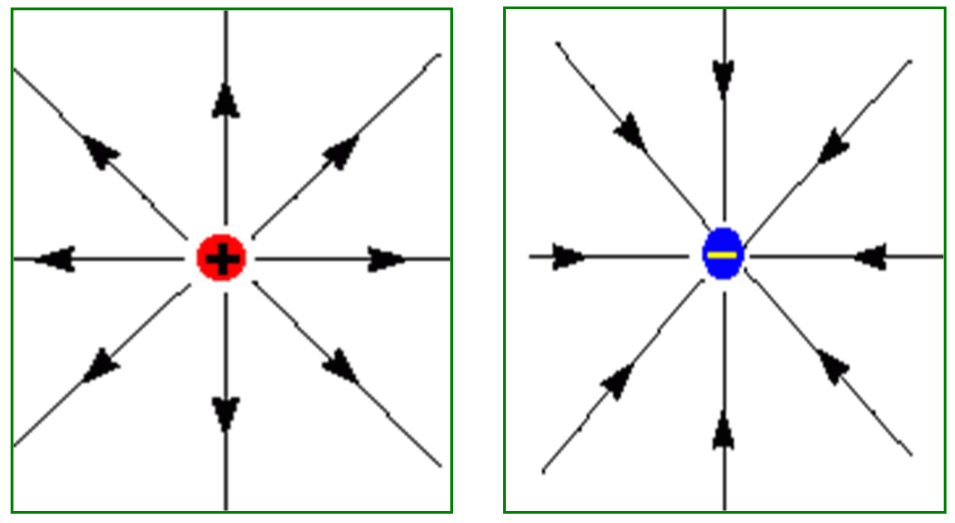
\includegraphics[width=0.80\textwidth]{Elektrisches Feld .png}
    \caption{Links nach außen gerichteter Feldvektor, rechts nach innen gerichteter Feldvektor.}
\end{figure}
Elektrische Feldlinien starten an positiven und enden an negativen Ladungen. 
Bei gleichen Ladungen stoßen sich die Feldlinien ab, bei entgegengesetzten Ladungen enden sie in der negativen Ladung.
Feldlinien können niemals bei der Ladung enden von der sie herkommen (keine geschlossenen Feldlinien).
\begin{figure}[H]
    \centering
    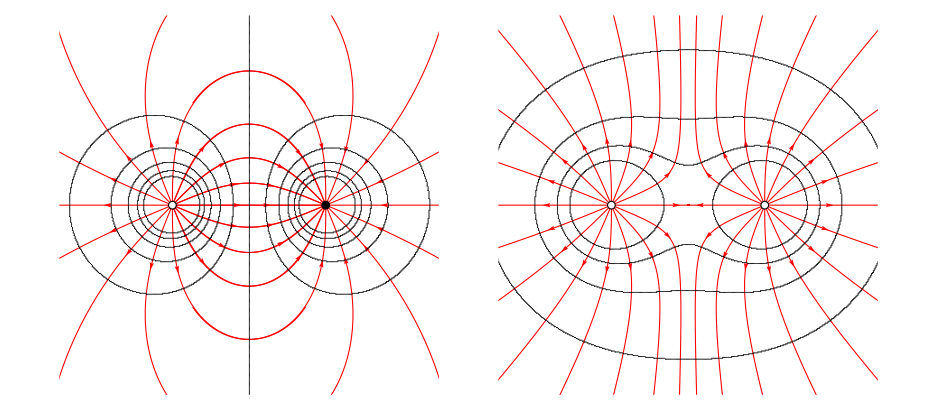
\includegraphics[width=0.80\textwidth]{Elektrisches Feld Ladungen.png}
    \caption{Links zwei entgegengesetzt Ladungen, Rechts zwei identische Ladungen}
\end{figure}

\subsection{Elektrische Leiter in einem elektrischen Feld}
Das Elektrische Feld im inneren eines geschlossenen Leiters ist immer null.
An der Oberfläche eines Leiters steht das elektrische Feld immer senkrecht zur Oberfläche.
Ein Beispiel für diese Eigenschaften ist der Faraday-Käfig.
\begin{figure}[H]
    \centering 
    \includegraphics[width=0.50\textwidth]{faraday käfig.png}
    \caption{Zu sehen ist, dass im inneren des Leiters das Elektrische Feld Null ist und die Feldlinien senkrecht zur Oberfläche stehen.}
\end{figure}

\subsection{Das Superpositionsprinzip}
Will man ein Elektrisches Feld für mehrere Ladungen berechen, so ergibt sich das resultierende Feld und Kraft 
durch die Überlagerung der einzel Felder.
Für das Elektrische Feld der Ladungen $q_i$ am Punkt $P$ (die Probeladung) gilt:
\begin{align}
    E_\mathrm{P}=k\cdot \sum_{i=1}^n \frac{q_i}{|\vec{r_i}|^2}\hat{r_i}
\end{align}
Die Kraft auf die Probeladung $q$ ergibt sich dann als:
\begin{align}
    \vec{F}=q\vec{E}_\mathrm{P}
\end{align}


\subsection{Spannung}
Die elektrische Spannung ist Arbeit im elektrischen Feld. Ihre Einheit ist $[\vec{E}]=\frac{\mathrm{V}}{\mathrm{m}}$.
Die Ladung q befindet sich in einem elektrischen Feld $\vec{E}(\vec{r})$ und soll von $\vec{r_1}$ nach $\vec{r_2}$ verschoben
werden. Dafür ist die Arbeit:
\begin{align}
    W&=\int_{\vec{r_1}}^{\vec{r_2}}\vec{F}(\vec{r})\,d\vec{r}\\
    &=q\int_{\vec{r_1}}^{\vec{r_2}}\vec{E}(\vec{r})\,d\vec{r}
\end{align}
notwendig.\\

\noindent Der Ausdruck des Integrals des Elektrischen Feldes wird als Potentialdifferenz ($U_2-U_1$) bezeichnet:
\begin{align}
    \int_{\vec{r_1}}^{\vec{r_2}}\vec{E}(\vec{r})\,d\vec{r}=U_2-U_1
\end{align}
Somit ergibt sich für die Arbeit $W$ im elektrostatischen Feld:
\begin{align}
    W&=q\int_{\vec{r_1}}^{\vec{r_2}}\vec{E}(\vec{r})\,d\vec{r}=q(U_2-U_1)
\end{align}
Die Arbeit in einem elektrostatischen Feld ist vom Weg unabhängig und hängt
nur vom Anfangspotential \( U_1 \) und Endpotential \( U_2 \) ab.
Ist dies gegeben, so handelt es sich um ein \textbf{konservatives Kraftfeld}.\\

\noindent In einem solchen Feld existiert ein Potential \( U(\vec{r}) \), aus dem das elektrische Feld berechnet werden kann:
\begin{align}
\vec{E}(\vec{r}) = -\vec{\nabla} U(\vec{r})
\end{align}

Diese Gleichung beschreibt, wie stark und in welche Richtung sich das Potential ändert.
Das \textbf{Minuszeichen} zeigt an, dass das elektrische Feld in Richtung des stärksten Abfalls des Potentials zeigt.\\

\noindent Das Potential einer Punktladung $Q$ lässt sich über 
\begin{align}
    U(\vec{r})=k\cdot\frac{Q}{r}\, \left(+U_0\right)
\end{align}
berechnen.\\

\noindent Die Spannung (Potentialdifferenz) ist nur definiert zwischen zwei Punkten.
Für die Potentialdifferenz zwischen Punkt $A$ und Punkt $B$ gilt:
\begin{align}
    U_{AB}=U(\vec{r_2})-U(\vec{r_1})=\frac{Q}{4\pi\varepsilon_0}\left(\frac{1}{r_2}-\frac{1}{r_1}\right)
\end{align}
Ist das Potential gleich Null, so liegt der Punkt im unendlichen. 
\begin{align}
    \lim_{r\to\infty}U(\vec{r})=0
\end{align}
Also: umso weiter weg man von einer Punktladung geht, desto kleiner wird das Potential.

\subsection{Plattenkondensator}
\begin{figure}[H]
    \centering
    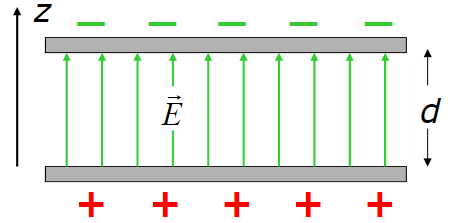
\includegraphics[width=0.6\textwidth]{Plattenkondensator.png}
    \caption{Der Aufbau eines Plattenkondensators mit der $z$-Achse}
\end{figure}
Bei einem Plattenkondensator gibt es zwei parallele, gegengesetzt geladene Metallplatten im Abstand $d$.
Diese bilden einen Kondensator aus.
Die Feldvektoren stehen senkrecht auf der positiv geladenen Platte und sind senkrecht auf die negative Platte gerichtet.
Sie entsprechen dem Einheitsvekor in $z$-Richtung:
\begin{align}
    \vec{E}\,||\,\hat{e}_z
\end{align}
Zudem ist das Elektrische Feld konstant, also homogen (überall gleich stark und gleiche Richtung) im inneren des Kondensators.
\begin{align}
    \vec{E}(\vec{r})=\vec{E}_0=const.\label{Plattenkondensator homogen}
\end{align}
Die Potenzialdifferenz (Spannung) zwischen den Platten ist:
\begin{align}
    \Delta U&=\int_0^d E(z)\,dz\\
    &=E_0\int_{0}^{d}dz\label{E_0 rausziehen}\\
    &=E_0\cdot d
\end{align}
Schritt~\ref{E_0 rausziehen} geht auf Grund des homogenen Feldes innerhalb des Plattenkondensators (siehe Formel~\ref{Plattenkondensator homogen}).
Für das Feld folgt damit:
\begin{align}
    E_0=\frac{\Delta U}{d}
\end{align}
Für die Einheit des elektrischen Feldes gilt $[E]=\frac{\mathrm{V}}{\mathrm{m}}$.
Bei Platten endlicher länge, ist das Feld am Rand (also Rechts und links) inhomogen.

\subsubsection{Beweis für die homogenität des elektrischen Feldes des Plattenkondensators}
Man betrachte eine Probeladung $q$ die sich im Abstand $a$ über einer großen Fläche mit 
gleichmäßiger Flächenladungsdichte $\sigma$ befindet.\\
Diese Fläche trägt eine Ladung:
\begin{align}
    dQ=\sigma\cdot da
\end{align}
Die Probeladung spürt eine Kraft durch das elektrische Feld dieser Fläche.
\begin{align}
    dF=k\cdot\frac{q\cdot dQ}{b^2}=k\cdot \frac{q\cdot \sigma\cdot dA}{b^2}
\end{align}
dabei ist $b$ der Abstand zwischen Probeladung und einem infinitesimal kleinen Flächenelement $dA$.\\

\noindent Nun zerlegt man die Kraft in zwei Richtungen. 
Einmal senkrecht zur Fläche (wirksame Kaft)
\begin{align}
    dF_s=dF\cdot \cos \alpha
\end{align}
und einmal Parallel zur Fläche (Symmetrische Kraft, diese hebt sich auf.)
\begin{align}
    dF_p=dF\cdot \sin \alpha=0
\end{align}
Die Symmetrische Kraft hebt sich auf, da alle horizontalen Anteile der Kräfte von gegenüberliegenden
Flächenelementen kompensiert werden.\\

\noindent Nun wird ein Ring mit Radius $r$ und Breite $dr$ betrachtet. Für die Fläche gilt:
\begin{align}
    dA=2\pi r\,dr
\end{align}
Es gelten folgende Beziehungen:
\begin{align}
    r=a\cdot\tan\alpha\\
    b=\frac{a}{\cos\alpha}
\end{align}
Die Ableitung von $r$ nach $\alpha$:
\begin{align}
    \frac{dr}{d\alpha}=\frac{a}{\cos^2\alpha}
\end{align}
Eingesetzt in $dF_s$ mit anschließendem Umformen und Integrieren gibt:
\begin{align}
    F=\frac{q\cdot \sigma}{2\varepsilon_0}
\end{align}
Somit haben wir bewiesen, dass die Kraft unabhängig von $a$ ist und somit konstant ist.
Somit ist das Feld eines idealen Plattenkondensators homogen.\\

\noindent Für die Kraft zweier Platten mit Ladung $Q$ gilt:
\begin{align}
    E=\frac{\sigma}{\varepsilon_0}=\frac{Q}{\varepsilon_0\cdot A}
\end{align}

\subsection{Kapazität}
Die Kapazität $C$ ist ein Maß dafür, wieviel Ladung man in einem Kondensator bei konstanter Spannung speichern kann.\\
Für das elektrische Feld gilt:
\begin{align}
    E&=\frac{U}{d}\\
    &=\frac{Q}{\varepsilon_0A}
\end{align}
Die Kapazität $C$ ist nun das Verhältnis zwischen der Ladung $Q$ und der Spannung $U$
\begin{align}
    C&=\frac{Q}{U}\\
    &=\frac{A\varepsilon_0}{d}
\end{align}
Diese Kapazität $C$ hängt nur von der Geometrie ab.
Ihre Einheit ist Farad $[C]=1\,\mathrm{F}=1\frac{\mathrm{A\,s}}{V}$
\begin{figure}[H]
    \centering
    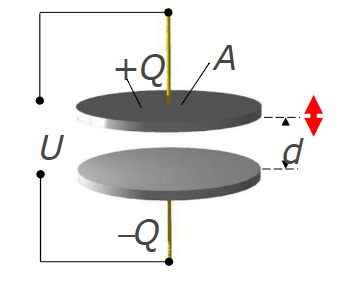
\includegraphics[width=0.40\textwidth]{aufbau plattenkondensator.png}
    \caption{Aufbau eines Plattenkondensators mit seinen relevanten Größen.}
\end{figure}

\subsection{Schaltzeichen eines Plattenkondensators}
\begin{figure}[H]
    \centering
    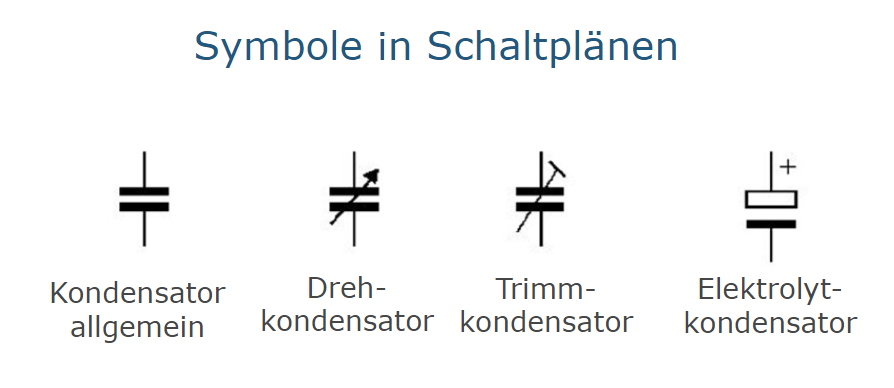
\includegraphics[width=0.8\textwidth]{Plattenkondensator schaltplan.png}
\end{figure}






\end{document}
